
\documentclass[preprint,12pt]{article}

\usepackage{hyperref, amsmath,amssymb,array, amscd, comment, color, datetime, graphicx}

%\usepackage{color}
%\usepackage[
%      colorlinks=true,
%%      linkcolor=darkblue,  
%      urlcolor=blue,    
%      filecolor=blue,     
%      citecolor=red,
%      pdfstartview=FitV,
%       bookmarksopen=true    
%      ]{hyperref}
%\usepackage[left=2.5cm,top=2.5cm,right=2.5cm,nohead]{geometry}



%%%%%%%%%%%%%%%%%%%%%%%%%%%%%%%%%%%%%%%%%%%%%%%%%%%%%%%%%%%%%%%%%
\input{/Users/Halmagyi/Dropbox/macro}
%%%%%%%%%%%%%%%%%%%%%%%%%%%%%%%%%%%%
\begin{document}
%%%%%%%%%%%%%%%%%%%%%%%%%%%%%%%%%%%%

\begin{center}
\fbox{DRAFT: \today,\ \currenttime}
\end{center}

\vspace{0.5cm}
\begin{center}
\baselineskip=13pt {\LARGE \bf{Notes on Bounding Box Construction \\
for Filtering Geographic Data}\\}
 \vskip1.5cm 
Nick Halmagyi\ 
 \vskip0.5cm
\textit{Laboratoire de Physique Th\'eorique et Hautes Energies,\\
Universit\'e Pierre et Marie Curie, CNRS UMR 7589, \\
F-75252 Paris Cedex 05, France}\\
\vskip0.5cm
nhalmagyi@gmail.com \\
\end{center}

%%%%%%%%%%%%%%%%%%%%%%%%%%%%%%%%%%%%
\section{Introduction}
%%%%%%%%%%%%%%%%%%%%%%%%%%%%%%%%%%%%

It is quite common in data science to manipulate geographic data in the form of the geodetic coordinates (latitude, longitude) of locations on the globe. It oftens happens that one has a single geographic location $S$ (the  source) and a set of geographic locations $\widehat{T}$ (the targets) and would like to answer one of the following questions:
\begin{enumerate}
\item return the closest $N$ targets in  $\widehat{T}$ to $S$
\item return all targets in $\widehat{T}$ within a given distance $d$ to $S$
\end{enumerate}
One can solve this by computing the distance $d(t_i, S)$ from every target to the source but for sufficiently large  $\widehat{T}$ this can be too slow for many purposes. A better solution is to make a bounding region $\cB$ around $S$ and compute the distance  $d(t_i,S)$ only for the $t_i \in \cB$. 

There are numerous ways to store a set of geographic locations in memory or on disk. For this bounding box algorithm useful one must utilize a fast method of filtering $\widehat{T}$ to those inside $\cB$. We have provided a \href{https://github.com/nickhalmagyi/BoundingBox}{python library} which does this. 

Geographic locations are typically given in the longitude-latitude coordinate system, so $\cB$ should be constructed from lines of equal latitude and lines of equal longitude. This results in $\cB$ which look roughly square close to the equator and a sort of curved quadrilateral when near the poles and finally a semi-circle when the box touches a pole.


%%%%%%%%%%%%%%%%%%%%%%%%%%%%%%%%%%%%
\section{Constructing the Bounding Box}
%%%%%%%%%%%%%%%%%%%%%%%%%%%%%%%%%%%%

We denote by $C_d$ the equidistant surface around $S$, it is the collection of points on the sphere which are exactly at a distance $d$ from $S$.  To construct the bounding box $\cB$, we need to determine the minimum and maximum values of latitide and longitude attained by $C_d$.

%%%%%%%%%%%%%%%%%%%%%%%%%%%%%%%%%%%%
\subsection{Haversine Formula}
%%%%%%%%%%%%%%%%%%%%%%%%%%%%%%%%%%%%
 
Two common methods to compute distances on the sphere are the Haversine and Vincenty metrics. Both metrics use the geodetic coordintae system, the Haversine formula assumes the earth is exactly spherical while the Vincenty metric inclues the oblateness of the earth. In this work we will use the Haversine formula as an approximation to the true distance between points.

The Haversine distance $d$ between two points $(\vphi_1,\lam_1)$ and $(\vphi_2,\lam_2)$ is 
 \be
 \sin^2\Blp \frac{d}{2R}\Brp= \sin^2\Blp \frac{\vphi_1-\vphi_2}{2} \Brp+ \cos \vphi_1\cos \vphi_2 \sin^2\Blp \frac{\lam_1-\lam_2}{2}\Brp
 \ee
 or more conveniently
 \bea
\cos \frac{d}{R} &=& \sin \vphi_1 \sin \vphi_2 + \cos (\lam_2 - \lam_1)   \cos \vphi_1 \cos \vphi_2\,.
 \eea
where $R$ is the radius of the sphere.
%%%%%%%%%%%%%%%%%%%%%%%%%%%%%%%%%%%%
\subsection{Maximum Latitude}
The maximum latitude on $C_d$ is attained when the longitude is the same as the longitude of $S$.  When two longitudes are equal 
 \be
 \lam_2=\lam_1
 \ee
the Haversine formula gives
\be
\varphi_2-\varphi_1 = \frac{d}{R}
\ee 


%%%%%%%%%%%%%%%%%%%%%%%%%%%%%%%%%%%%
\subsection{Maxmimum Longitude}

%%%%%%%%%%%%%%%%%%%%%%%%%%%%%%%%%%%%
\subsubsection{Ellipse}

To warm up to the computation of  the point of maximum longitude, we first look at an ellipse in $\RR^2$:
\be
a^2 x^2 + b^2 y^2 = 1 
\ee
and look for the maximum value of $x$.

We solve for $x$
\bea
x(y) &= & \frac{1}{a}\sqrt{(1- b^2 y^2 )} 
\eea
and compute the variation of $x$ w.r.t. $y$ 
\bea
x'(y) = \frac{1}{a}\frac{2b^2y}{(1- b^2 y^2 )}\,.
\eea 
The extremum of $x$ are of course at the point where $x'(y)=0$ and this is at $y=0$, in particular on the $x$-axis.


%%%%%%%%%%%%%%%%%%%%%%%%%%%%%%%%%%%%
\subsubsection{Back to the Sphere}
Given a section of equal distance $d$ from the source $S=(\varphi_1, \lam_1)$ we want to know the maximum longitudinal distance, i.e. the maximum value of $|\lam_2-\lam_1|$. These will be the east and west boundaries of the bounding box.

We first fix $d$ and $(\varphi_1, \lam_1)$ then look for the extremum of $\lam_2$ as a function of $\vphi_2$. It is convenient to change coordinates to
\be
\Lam= \cos\blp\lam_1-\lam_2(\vphi_2)\brp\,,\qquad \Psi = \sin \vphi_2
\ee
then the equations to be solved are
\bea
\csc \vphi_1\cos \frac{d}{R}&=&\cot \vphi_1 \Lam \sqrt{1-\Psi^2}  +\Psi \\
\cot \vphi_1\Lam \Psi &=& \sqrt{1-\Psi^2}
\eea
The solution is 
\bea
\Lam &=& \sec(\vphi_1 ) \sqrt{\cos^2 \blp\frac{d}{R}\brp - \sin^2 (\vphi_1)} \\
\Psi &=&\sec \blp\frac{d}{R}\brp  \sin \vphi_1
\eea

There is a branch point  in $\Lam$ at one of the following points:
\be
{\rm b.p.} \quad \vphi_1 \pm \frac{d}{R} = \pm \pi/2
\ee
which is where the bounding section touches the north(south) pole. At this point the maximum longitude reached is $\lam_2-\lam_1 = \pi/2$ which is half way around the globe (though not necessarily at the equator).


%%%%%%%%%%%%%%%%%%%%%%%%%%%%%%%%%%%%
\subsubsection{Equal  Latitude}

One can also consider a related but inequivalent question, which is to contruct the shortest distance between two points of equal latitude. This is slightly non-trivial since the great circle between two points does not follow lines of equal latitude unless both points are on the equator. Indeed in this interesting \href{http://janmatuschek.de/LatitudeLongitudeBoundingCoordinates}{blog post} the author realises the distinction between great circles and lines of constant latitude but mistakenly assumes that the maximum longitude is attained at the same latitude as the source $S$. 

To compute the distance between two points of equal latitude, we use the Haversine formula with
\be
\vphi_1=\vphi_2 = \vphi\,.
\ee
Then we find
\bea
d &=&  2R \sin^{-1} \Big| \cos \vphi   \sin \Blp \frac{\lam_1-\lam_2}{2}\Brp \Big|  \\
\Ra \quad |\lam_1 - \lam_2| &=& 2\left|\sin^{-1}\left[ \frac{\sin\left(\frac{d}{2R}\right)}{\cos(\varphi)}\right]\right|\,.
\eea
%The maximum longitudinal difference between two points is 
%\be
%|\lam_2-\lam_1|_{\rm max} = \pi
%\ee
%which occurs when
%\be
%\sin\left(\frac{d}{2R}\right)  = \cos(\varphi)\,.
%\ee
 


%%%%%%%%%%%%%%%%%%%%%%%%%%%%%%%%%%%%
\section{Constructing the Bounding Box}
%%%%%%%%%%%%%%%%%%%%%%%%%%%%%%%%%%%%

%%%%%%%%%%%%%%%%%%%%%%%%%%%%%%%%%%%%
\subsection{Pole Inside Bounding Box}

When the north or south pole is within a distance $d$ from $S$, the naive bounding box with cross the pole and therefore occupy all values of longitude. We proceed by constructing two bounding boxes, $\cB_f$ (the {\it front}) for the longitude region of width $\pi$ centered on $S$ and another $\cB_r$ (the {\it reverse}) for the remainding $\pi$-sized region. When the pole is is the north (south) pole, then the south(north) limit of $\cB_f$ is determined by the point on $C_d$ directly souht(north) of $S$ while the south(north) limit of the $\cB_r$is determined by the intersection of $C_d$ with the constant longitude lines of $\cB_f$. This is demonstrated in figure \ref{fig:bbox_reverse}:
\begin{figure}[bth!]
  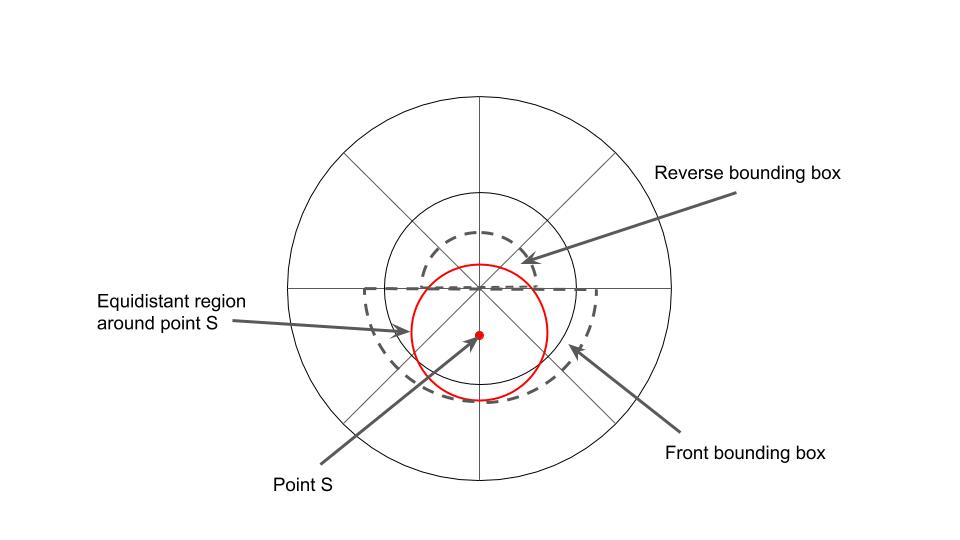
\includegraphics[width=\linewidth]{bbox_reverse}
  \caption{Construction of the two bounding boxes around $S$, where $S$ is near a pole on the sphere. The bounding boxes are marked by dashed lines and appear as hemispheres.  The equidistant surface is in red. The radial lines are at constant longitude, intersecting at the pole in the center of the figure.}
  \label{fig:bbox_reverse}
\end{figure}

%%%%%%%%%%%%%%%%%%%%%%%%%%%%%%%%%%%%
\bibliographystyle{/Users/Halmagyi/Dropbox/utphys} 
\bibliography{/Users/Halmagyi/Dropbox/myrefs}
%%%%%%%%%%%%%%%%%%%%%%%%%%%%%%%%%%%%

%%%%%%%%%%%%%%%%%%%%%%%%%%%%%%%%%%%%
\end{document}
%%%%%%%%%%%%%%%%%%%%%%%%%%%%%%%%%%%%
%%%%%%%%%%%%%%%%%%%%%%%%%%%%%%%%%%%%
